\hypertarget{introduction}{%
\section{Introduction}\label{introduction}}

The title and authors are included in the LaTeX preamble, but everything
that follows is written in markdown, including references and figures.

This is my introduction. This section automatically received the label
\texttt{introduction}. I can cite references in parentheses
\citep[see][]{bainbridgeResiliencyImageMemorability2020}. My favorite
paper is \citet{adrianBergerRhythmPotential1934}. I can crossref to
Figure \ref{paleblue} in section \ref{methods}.

\hypertarget{methods}{%
\section{Methods}\label{methods}}

I am describing methods. We did it like so:
\(\alpha=\beta * \frac{\pi}{2}\). This method was described in
\citet{michelDistinctContributions2021}.

Look again at that dot (Figure \ref{paleblue}). That's here. That's
home. That's us.

\begin{figure}
\centering
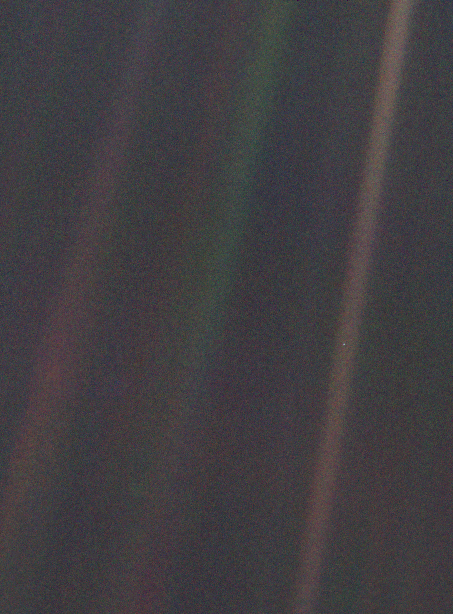
\includegraphics[width=\textwidth,height=0.5\textheight]{Pale_Blue_Dot.png}
\caption{A mote of dust suspended in a sunbeam. Downloaded from
https://en.wikipedia.org/wiki/Pale\_Blue\_Dot. \label{paleblue}}
\end{figure}
